\chapter{小手册} % Introduction chapter suppressed from the table of contents   


因故事点只是每个团队自己定义,无法用来作为组织级标准衡量规模,所以很多公司(尤其是银行)转用功能点来衡量软件开发规模。它不仅可用于公司内,也适用于行业标杆,例如验收测试缺陷数无法比较,但缺陷数除以功能点(规模)=
缺陷率,
便可以比较。功能点也适用于公司内或公司间结算,例如软件维护期里开发工作量变化很大,也难以事前预估,所以有些银行会按最终开发出来的功能点数结算使用部门付开发部的费用,减少争议。

虽然功能点分析源自70年代,但由于计算较复杂,一直未普及。针对这问题,国际功能点协会简化本来的功能点算法,推出简化功能点(SiFP)。虽然简化功能点数有偏差,但因敏捷迭代开发,每轮的规模不大,可以接受,所以越来越多团队开始从故事点转简化功能点,但由于不熟识功能点估算是从用户角度估算,而非从开发工程师的视角看,团队初次估算SiFP通常有误。下面是一些转简化功能点的常见问题:

\hypertarget{ux4eceux6545ux4e8bux70b9ux8f6cux7b80ux5316ux529fux80fdux70b9}{%
\subsection{从故事点转简化功能点}\label{ux4eceux6545ux4e8bux70b9ux8f6cux7b80ux5316ux529fux80fdux70b9}}

客户:我们以前一直使用故事点,为了更好做量化管理,我们新的项目开始使用简化功能点
- SiFP\\
我:好的,看一下你的估算表 。 。 。 。
为什么这两个功能要分成两个行为?\\
客户:这两个功能都挺复杂,估计需要很多开发工作量;我们以前用故事点估算时,也会分成两个故事点。\\
我:请注意,在功能点估算, 是否是一个行为,取决于它算不算是一个基本过程
如果俩行为互相依赖,不能单独作为基本过程,就不应该分开为2个功能点。很多团队刚开始用功能点,与你们一样,没有弄清楚基本过程的概念,还是从工程师的角度,估计开发时间的工作量来判断是一个功能还是两个功能?在故事点用这种方式估算习惯,但因为功能点是要同一个功能上需求,不能有功能点数的差异,所以不能用估计开发难易程度来判断。\\
客户:可否举个实例?\\
我:以网约车为例,是否可以分成以下''行为``:

%Screenshotfrom20221219021057.png

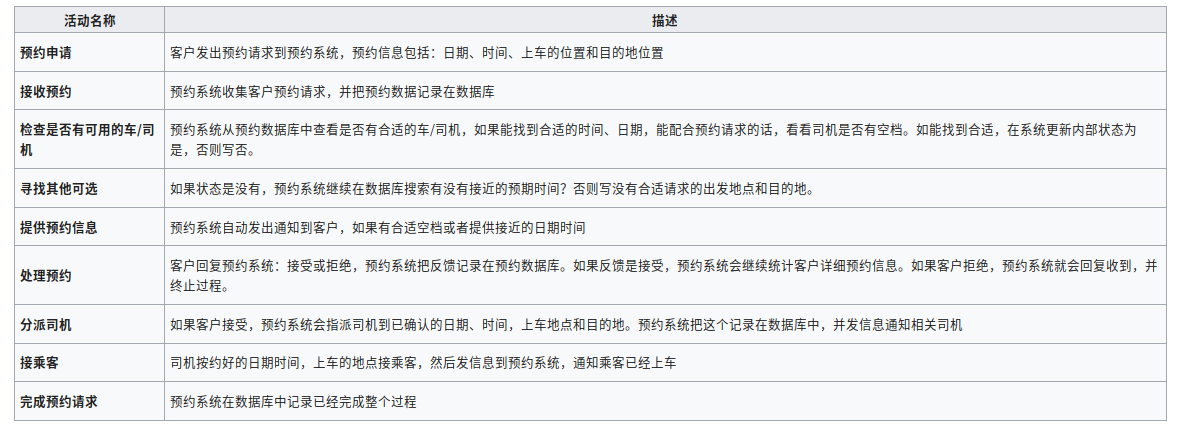
\includegraphics[width=10cm]{Screenshotfrom20221219021057.png}

客户:是的,而且每个行为都要花一定开发工作量。\\
我:其实只有4个行为,因头5个,和最后2个都要合并才可以成行为(详见附件)。
如果要能独立成行为,必须符合基本过程条件。
基本过程不是随便定的,它有规则,比如从网约车案例我们可以看到,``预约申请''本身不能算一个基本过程,虽然预约申请可能要很复杂的开发工作,但是因为它不能独立存在,必须依赖其它的行为才算完整。\\
例如,某公司财务系统有打印支票功能(用来付供应商),你觉得打印支票本身是否算基本过程?\\
客户:听完你网约车例子,应该不算;因打印支票只是付款流程的一个可选部分。\\
我:正确、算实体也应使用同样概念。例如,某人事管理系统,除了管理职工信息外,还有员工家属信息,因家属信息必须关连到员工信息,不能独立存在,所以家属信息本身不算是一个实体。你是否觉得你这表里的某些实体应合并?\\
客户:听完你的解释,同意我们这次计算有些实体应合并。\\
我:你们的功能点估算表没有明确区分新的迭代怎么处理变更与删除。
也没有明确动态功能点与静态功能点。\\
客户:我们表中有计算每次迭代的总功能点数。\\
我:你们可能有算每迭代的功能点,但难以看清后面迭代对应之前的变化。动态功能点是用来估算本本迭代的工作量,而静态功能点就是迭代后产品的功能点数。而且应该用表格形式把变更和删除累加在原本上一轮的功能上面,才可以更好看到迭代与迭代之间,功能上的变化。(详见附件例子)\\
所以不要误以为可以像之前故事点估算,利用两页纸,写上各种复杂程度的故事点例子便可。国际功能点手册里包含很多计算实例,来解释功能点计算,才能确保对同一套需求,各人(依据用户的角度)才能估算出同样的功能点数。我刚刚的例子全都可以从国际功能点手册里找到,你们不需要再发明车轮(reinvent
the wheel)。学功能点估算与写程序类似,必须多动手试。

建议你们读完网约车识别基本过程例子后,再读潜水学校两实例:

\begin{enumerate}
\tightlist
\item
  首次开发
\item
  增强功能与维护 (Enhancement)
\end{enumerate}

觉得已经把握好功能点计算原理,可尝试练习3+4,同样是首次开发+
增强功能与维护。

\hypertarget{ux603bux7ed3}{%
\subsubsection{总结}\label{ux603bux7ed3}}

虽然简化功能点比传统国际功能点NESMA简单,容易学,但开发人员容易还是用工程师的视角来估算(本应用用户的视角),导致计算错误。所以要多看案例,并做练习才能把握(能参加培训会更好)。因简化功能点不考虑实体/行为的复杂度,个别估算与传统功能点有偏差(详见附件),但因SiFP是取高中低中间值计算,所以多次估算的平均值能近似IFPUG/NESMA
估算值,尤其适用于敏捷多次迭代估算。

\hypertarget{ux9644ux4ef6}{%
\section{附件}\label{ux9644ux4ef6}}

\hypertarget{ux7b80ux5316ux529fux80fdux70b9sifp-ux7b80ux4ecb}{%
\subsection{简化功能点(SiFP)
简介}\label{ux7b80ux5316ux529fux80fdux70b9sifp-ux7b80ux4ecb}}

 \textbf{它是做什么的?} \\
应用软件开发的客户需求可分成三类:

\begin{enumerate}
\tightlist
\item
  功能性需求
\item
  技术需求
\item
  质量需求
\end{enumerate}

第二类和第三类归为非功能性需求。功能点主要是针对功能性需求,目的是提供对客户有意义的功能点数,来客观地衡量软件规模。

 \textbf{该如何去做?} \\
简化功能点(SiFP)主要两类度量:

\begin{enumerate}
\tightlist
\item
  数据功能 - 实体 (逻辑文件 Logical File)
\item
  事务功能 - 行为(基本过程 Elementary Process)
\end{enumerate}

%\href{文件:功能点计数过程.jpg}{500px}

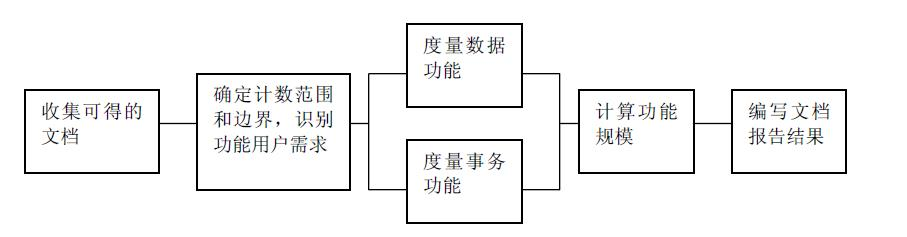
\includegraphics[width=10cm]{功能点计数过程.jpg}

\hypertarget{ux7b80ux5316ux529fux80fdux70b9ux4f30ux7b97ux6b65ux9aa4}{%
\subsubsection{简化功能点估算步骤:}\label{ux7b80ux5316ux529fux80fdux70b9ux4f30ux7b97ux6b65ux9aa4}}

\begin{enumerate}
\tightlist
\item
  确定功能点分析类型
\item
  识别分析范围和应用边界
\item
  计算数据类型功能点(Data Function)
\item
  计算交易类型功能点(Transaction Function)
\item
  计算功能点
\end{enumerate}

\hypertarget{ux4e09ux79cdsifpux8ba1ux7b97ux7c7bux578b}{%
\subsubsection{1:三种SiFP计算类型}\label{ux4e09ux79cdsifpux8ba1ux7b97ux7c7bux578b}}

\begin{itemize}
\tightlist
\item
  开发(Development )
\end{itemize}

\begin{description}
\item[]
\begin{description}
\tightlist
\item[]
DSFP = ADD + CFP
\end{description}
\end{description}

\begin{itemize}
\tightlist
\item
  应用 (Application or Baseline after the initial development)
\end{itemize}

\begin{description}
\item[]
\begin{description}
\tightlist
\item[]
ASFP = ADD
\end{description}
\end{description}

\begin{itemize}
\tightlist
\item
  更新/增强功能与维护 (Enhancement)
\end{itemize}

\begin{description}
\item[]
\begin{description}
\tightlist
\item[]
ESFP = ADD + CHG + DEL + CFP
\end{description}
\end{description}

%Screenshotfrom20221219021338.png

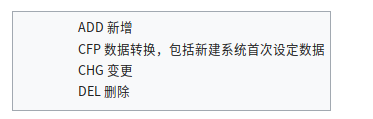
\includegraphics[width=10cm]{Screenshotfrom20221219021338.png}

\hypertarget{ux8bc6ux522bux5206ux6790ux8303ux56f4ux548cux5e94ux7528ux8fb9ux754c}{%
\subsubsection{2:识别分析范围和应用边界}\label{ux8bc6ux522bux5206ux6790ux8303ux56f4ux548cux5e94ux7528ux8fb9ux754c}}

例子:用虚线标示系统边界:\\
%\href{文件:功能点计数P62_2.0.jpg}{500px}\\

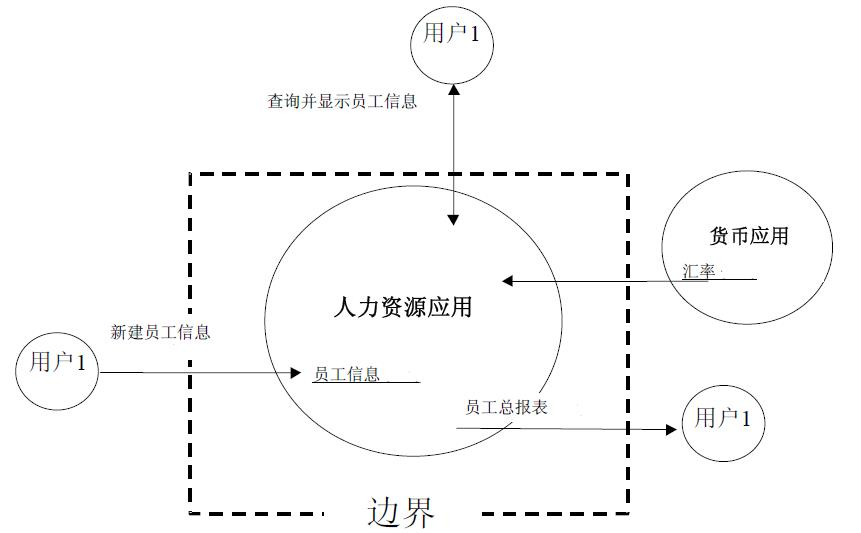
\includegraphics[width=10cm]{功能点计数P6220.jpg}


\hypertarget{ux8ba1ux7b97ux903bux8f91ux6587ux4ef6ux6570}{%
\subsubsection{3:计算逻辑文件数}\label{ux8ba1ux7b97ux903bux8f91ux6587ux4ef6ux6570}}

\begin{itemize}
\tightlist
\item
  关于计算规则,详见"逻辑文件"
\end{itemize}

\hypertarget{ux8ba1ux7b97ux57faux672cux8fc7ux7a0bux6570}{%
\subsubsection{4:计算基本过程数}\label{ux8ba1ux7b97ux57faux672cux8fc7ux7a0bux6570}}

\begin{itemize}
\tightlist
\item
  关于计算规则,详见"基本过程"
\end{itemize}

\hypertarget{ux8ba1ux7b97ux529fux80fdux70b9}{%
\subsubsection{5:计算功能点}\label{ux8ba1ux7b97ux529fux80fdux70b9}}

\begin{itemize}
\tightlist
\item
  每个逻辑文件 = 7.0 简化功能点
\item
  每个基本过程 = 4.6 简化功能点
\end{itemize}

\hypertarget{ux903bux8f91ux6587ux4ef6-logical-file}{%
\subsection{逻辑文件 Logical
File}\label{ux903bux8f91ux6587ux4ef6-logical-file}}

\textbf{(下面在计算实例里简称``实体'',方便理解)}

\begin{itemize}
\tightlist
\item
  用来储存内部或外部数据,是用户可识别的逻辑相关的数据组或控制信息组,在被度量应用边界内部维护。
\end{itemize}

\begin{description}
\tightlist
\item[]
(\textbf{用户可识别} -
指数据或事务需求是被用户和软件开发人员双方共同认同并理解的。
例如:用户和软件开发人员双方都认同人力资源应用有维护和存储员工信息的功能。)
\end{description}

\hypertarget{ux6ce8ux610f}{%
\paragraph{注意}\label{ux6ce8ux610f}}

逻辑文件包括两类不同的用户需求数据:

\begin{enumerate}
\tightlist
\item
  功能性数据
\item
  非功能性数据
\end{enumerate}

功能性数据是用来满足用户功能需求的数据。例如,销售、银行账号、供应商、人员等信息。\\
非功能数据主要是为了满足易用性(支撑下拉菜单所需的数据,可输入数据的上下范围等);或性能方面(用于查询数据的索引index);或可维护性(配置参数)。\\
只有第一类功能性数据才算是逻辑文件。\\

\hypertarget{ux57faux672cux8fc7ux7a0b-elementary-process}{%
\subsection{基本过程 Elementary
Process}\label{ux57faux672cux8fc7ux7a0b-elementary-process}}

基本过程是对用户有意义的最小活动单元。例如:添加员工的用户需求包括建立工资和家属信息。只有添加所有员工信息,才能创建员工信息记录。单独添加一些信息使添加员工业务处于不持续状态,只有员工工资和家属信息都添加后,这个活动单元才能完成且业务处于稳定状态。

\hypertarget{ux8bc6ux522bux57faux672cux8fc7ux7a0b}{%
\subsubsection{识别基本过程}\label{ux8bc6ux522bux57faux672cux8fc7ux7a0b}}

为了识别基本过程,需要执行以下活动:

\begin{itemize}
\tightlist
\item
  把功能用户需求分解为最小活动单元,使其满足下面条件:

  \begin{itemize}
  \tightlist
  \item
    对用户有意义\\
    例如:功能用户需求要求在应用中添加新员工的能力。\\
  \item
    构成一个完整的事务\\
    例如:用户定义的员工信息包括工资和家属信息。如果家属人数大于零,添加员工信息时必须包括家属信息。本例中,添加员工信息(不包括添加地址、工资和家属信息)不满足本规则。\\
  \item
    自包含\\
    例如:除非输入所有的必需信息并且完成所有处理步骤,如验证、计算、更新ILFs,添加过程才是自包含的。\\
  \item
    让应用程序的业务保持持续状态\\
    例如:添加员工的用户需求包括建立工资和家属信息。只有添加所有员工信息,才能创建员工信息记录。单独添加一些信息使添加员工业务处于不持续状态,只有员工工资和家属信息都添加后,这个活动单元才能完成且业务处于持续状态。\\
  \end{itemize}
\end{itemize}

识别活动单元为基本过程需要满足以上所有规则。\\

\hypertarget{ux8bc6ux522bux57faux672cux8fc7ux7a0bux4e3bux8981ux76eeux7684}{%
\subsubsection{识别基本过程主要目的}\label{ux8bc6ux522bux57faux672cux8fc7ux7a0bux4e3bux8981ux76eeux7684}}

基本过程的主要目的可识别为下列情形的一种:

\begin{itemize}
\tightlist
\item
  改变应用行为
\item
  维护一个或多个ILFs
\item
  呈现信息给用户
\end{itemize}

\hypertarget{ux5b9eux4f8b1ux8bc6ux522bux57faux672cux8fc7ux7a0b-ep-elementary-process}{%
\section{实例1:识别基本过程 (EP elementary
process)}\label{ux5b9eux4f8b1ux8bc6ux522bux57faux672cux8fc7ux7a0b-ep-elementary-process}}

下面是某预约网约车过程:

%\href{文件:sifp_p50图.jpg}{600px}

\includegraphics[width=10cm]{sifpp50图.jpg}

\begin{enumerate}
\tightlist
\item
  预约申请
\item
  接收预约
\item
  检查是否有可用的车/司机
\item
  寻找其他可选
\item
  提供预约信息
\item
  处理预约
\item
  分派司机
\item
  接乘客
\item
  完成预约请求
\end{enumerate}

\hypertarget{ux5206ux6790ux80fdux5426ux6ee1ux8db3ux6240ux6709-ep-ux8bc6ux522bux89c4ux5219ux5224ux65adux80fdux5426ux72ecux7acbux6210ux4e3aux57faux672cux8fc7ux7a0b-ep-elementary-processux90e8ux5206ux4f8bux5b50}{%
\subsection{分析能否满足所有 EP 识别规则,判断能否独立成为基本过程 (EP
elementary
process),部分例子}\label{ux5206ux6790ux80fdux5426ux6ee1ux8db3ux6240ux6709-ep-ux8bc6ux522bux89c4ux5219ux5224ux65adux80fdux5426ux72ecux7acbux6210ux4e3aux57faux672cux8fc7ux7a0b-ep-elementary-processux90e8ux5206ux4f8bux5b50}}

\hypertarget{ux9884ux7ea6ux7533ux8bf7}{%
\subsubsection{预约申请}\label{ux9884ux7ea6ux7533ux8bf7}}

\begin{enumerate}
\tightlist
\item
  是否对用户有意义,客户功能需求的一部分?\textbf{是}
\item
  是否构成一个完整的事务?\textbf{否}:预约申请本身不是一个完整的交易,因为过程必须也包括预约请求信息,收到其它可选的档期这些步骤,都不可以分离。
\item
  是否自包含,可以独立存在?\textbf{否}:例如,接受预约申请;查看是否有档期,查看有没有其它接近的档期等,都是一些必须的相关步骤去完成这个基本过程。
\item
  是否让应用程序达到稳定状态?\textbf{否}:整个业务需求只能在收到预约信息,发送、接受、处理、反馈给客户才算是完成稳定状态。
\end{enumerate}

\hypertarget{ux5206ux6d3eux53f8ux673a}{%
\subsubsection{分派司机}\label{ux5206ux6d3eux53f8ux673a}}

\begin{enumerate}
\tightlist
\item
  是否对用户有意义,客户功能需求的一部分?\textbf{是}
\item
  是否构成一个完整的事务?\textbf{是}:分配到司机是一个完整的交易,包括收到司机的确认,把信息记录在系统中并通知司机。
\item
  是否自包含,可以独立存在?\textbf{是}:分配到司机本身可以独立存在。
\item
  是否让应用程序达到稳定状态?\textbf{是}:因为当司机被分配后,是完全满足业务的需要。
\end{enumerate}

\hypertarget{ux63a5ux4e58ux5ba2}{%
\subsubsection{接乘客}\label{ux63a5ux4e58ux5ba2}}

\begin{enumerate}
\tightlist
\item
  是否是客户功能需求?\textbf{是}
\item
  交易是否完整?\textbf{否}:接乘客本身不算一个完整的交易,因为预约系统必须也记录这个信息。
\item
  是否自包含,可以独立存在?\textbf{否}:确认预约申请是下面一个必须执行的过程,来完成这个基本过程。
\item
  是否让应用程序达到稳定状态?\textbf{否}:整个业务需求只能在和预约系统确认沟通,已经接到乘客,然后系统也把记录更新到预约系统才算完成。
\end{enumerate}

%Screenshotfrom20221219021522.png

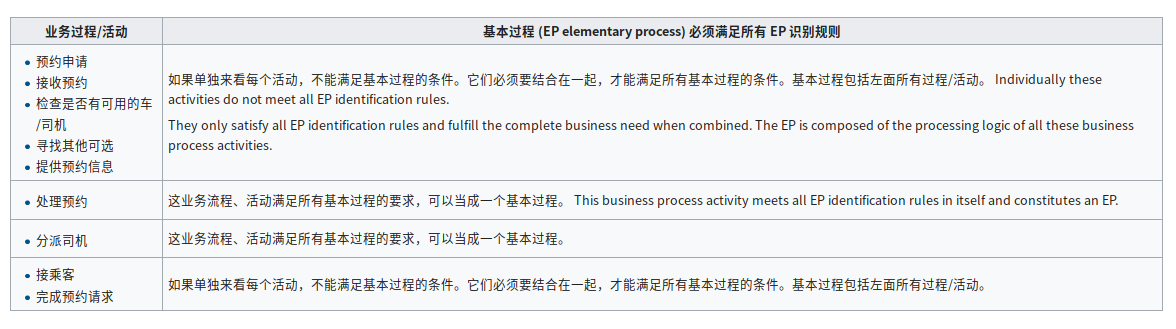
\includegraphics[width=10cm]{Screenshotfrom20221219021522.png}

\hypertarget{ux6f5cux6c34ux5b66ux6821ux5f00ux53d1ux9879ux76ee-example-diving-school-development-project}{%
\subsection{1.潜水学校:开发项目 EXAMPLE Diving School: Development
Project}\label{ux6f5cux6c34ux5b66ux6821ux5f00ux53d1ux9879ux76ee-example-diving-school-development-project}}

\hypertarget{ux63cfux8ff0}{%
\subsubsection{描述}\label{ux63cfux8ff0}}

一所潜水学校需要一套用来管理合同员工(教练)、设施、轮班工作的系统。目的:有效地管理教练在潜水设施和几艘旅游潜水船上有关潜水课程/短途潜水的轮班工作。A
diving school requires a system for managing their information:
contractors, facilities, working shifts to effectively manage the
coverage of shifts by the instructors that are available at the diving
facilities and aboard several boats for touristic dives and diving
courses.

\hypertarget{ux529fux80fdux9700ux6c42}{%
\subsubsection{功能需求}\label{ux529fux80fdux9700ux6c42}}

\hypertarget{rf01}{%
\paragraph{RF01}\label{rf01}}

为处理教练保险单文件,并符合法例,学校需要为每个合同员工储存以下资料:

\begin{itemize}
\tightlist
\item
  序列号(独特,作为索引, 不能重复)
\item
  姓名
\item
  居住地址
\item
  城镇
\item
  邮政编码
\item
  电话号码
\item
  是否持有航海执照
\end{itemize}

To handle the documentation for the insurance policies of the
instructors and to be in compliance with the current legislation, the
school needs to store the following information for each Contractor:

\begin{itemize}
\tightlist
\item
  unique serial number
\item
  first name and last name,
\item
  address of residence,
\item
  town of residence,
\item
  postal code of residence,
\item
  telephone number,
\item
  whether in possession or not of nautical licence.
\end{itemize}

为了跟踪每个合同员工的``职业生涯'',学校决定给予他们以下分类:

\begin{enumerate}
\tightlist
\item
  ``潜水长''
\item
  ``助理教练''
\item
  ``教练''
\end{enumerate}

In order to keep track of the 'career' of each Contractor, the school
decided to associate with them a category, which can take the following
values:

\begin{enumerate}
\tightlist
\item
  "Dive-master"
\item
  "Assistant Instructor"
\item
  "Instructor"
\end{enumerate}

这些分类是固定的,并不会随着时间而转变:每个合同员工会按顺序分配到合适的类别,代表个人``职业生涯''的发展(例如,一个新员工开始是``潜水长'',随着时间的推移,他会成为``教练'')。These
values are fixed and are not expected to change over time; they can be
assigned to each Contractor sequentially and represent the progress of
'careers' within the school (e.g. a new employee starts as "Dive-master"
and advances over time to become "Instructor").

使用表单输入,显示,编辑和删除合同员工的数据。会有一个独立列表框,显示序列号、名和姓
(但没有附件明细),来选择要编辑、删除或详细查看的是哪位员工的数据。

Forms must be created for entry, display, editing and deletion of
Contractor's data. In order to select the occurrence of data to edit,
delete or view in detail, there will be an independent list box of items
without accessory details: Serial number, Name and Surname.

用功能键激活所有的功能,并最终产生一个结果或错误信息。``删除合同员工''只是在逻辑上删除,没有数据会被物理删除,但会被标记为作废。只要有与其相关的工作班次,合同员工就不能被删除。

A function key will activate all the functions, and eventually generate
an error/outcome message. The deletion of a Contractor is only a logical
one: no data will be physically deleted, but will be labeled as
obsolete. A Contractor cannot be deleted as long as there are working
shifts associated with it.

\hypertarget{rf02}{%
\paragraph{RF02}\label{rf02}}

学校还需要管理设施(``潜水''、``船''或``橡皮艇-RD''),每一个设施都有独特的友好名称(例如:``潜水莫格利亚
diving\_moneglia''、``潜水帕拉 diving\_palau''、``蓝箭艇
blue-arrow-boat''、``格里大艇 goletta-boat''、``嘉莉花RD
Genova\_RD''等等)。

The school also needs to manage the Facilities ("diving", "boat" or
"rubber dinghy - RD"), to each of which a unique friendly name is
associated (for example: ``diving\_moneglia'', ``diving\_palau'',
``blue-arrow-boat'', ``goletta-boat'', ``Genova\_RD'' and so on).

对于每种类型的设施,必须存储以下信息:

\begin{itemize}
\tightlist
\item
  设施识别名(独特,作为索引,不能重复)
\item
  描述
\item
  类型
\item
  它能容纳的人数
\item
  可用汽缸数
\item
  是否有厕所
\item
  是否有饮用水储备
\end{itemize}

For each type of facility, the following information must be stored:

\begin{itemize}
\tightlist
\item
  unique identifier of the Facility
\item
  description
\item
  type
\item
  number of people it can host
\item
  number of available cylinders
\item
  presence or absence of portable toilet
\item
  presence or absence of drinking water reserve.
\end{itemize}

必须创建表单来输入、显示、编辑和删除设施数据;如果有被分派到轮班,就不能删除设施。使用独立的列表(不显示附件细节),以便选择要编辑、删除或详细查看的数据,列表只展示:标识名称、描述、类型\\
用功能键来激活某功能,并最终生成错误或结果信息。

Forms must be created for entry, display, editing and deletion of
Facility data; a Facility cannot be deleted if there are active shifts.
In order to select the occurrence of data to edit, delete or view in
detail, there will be an independent display of the list of items
without accessory details: Identifier, Description, Type. A function key
will activate all the functions, and eventually generate an
error/outcome message.

\hypertarget{rf03}{%
\paragraph{RF03}\label{rf03}}

最后,为了有效管理分派轮班(shift)的覆盖范围,学校需要处理合同员工以下轮班(shift)信息:

\begin{itemize}
\tightlist
\item
  工作轮班识别名(独特,作为索引,不能重复)
\item
  可用的合同员工编号(使用下拉框挑选)
\item
  提供本轮班可用的日期
\item
  可用期的开始日期
\item
  可用期的结束日期
\item
  首选设施(使用下拉框挑选)
\item
  状态(最初预设置为``预计轮班'')
\end{itemize}

Lastly, in order to effectively manage shifts coverage, the school needs
to handle the following shift availability information of Contractors:

\begin{itemize}
\tightlist
\item
  unique identifier of the working shift
\item
  serial number of the Contractor who is available (using a combo-box),
\item
  date on which availability was provided,
\item
  start date of the availability period,
\item
  end date of the availability period,
\item
  preferred facility (using a combo-box)
\item
  status (initially set to "tentative shift").
\end{itemize}

必须创建表单来输入、显示、编辑和删除轮班(shift)的有效信息。为了方便选择对哪些数据进行编辑、删除或查看详细信息,会独立显示没有附件细节的数据列表(如,不显示可用性标识号,合同员工序列号)。用功能键将激活这功能,并最终生成错误/或结果信息。

Forms must be created for entry, display, editing and deletion of Shift
availability data. In order to select the occurrence of data to edit,
delete or view in detail, there will be an independent display of the
list of items without accessory details: Availability identifier,
Contractor serial number. A function key will activate all the
functions, and eventually generate an error/outcome message.

\hypertarget{rf04}{%
\paragraph{RF04}\label{rf04}}

每个合同员工可以提供不止一个可用轮班(availability),每一个轮班最初都设定为``预计轮班tentative
shift''状态。当分配协调各合同员工的可用轮班作为一个``轮班(shift)''内的可用资源时,秘书处在一个``分配轮班
assigned
shift''内使用特定命令选择(转换)所需的可用轮班(availability),她可以更改潜水期的开始和结束日期,并可以将之设定为``分派轮班''状态。删除``分派轮班''与删除``预计轮班''的功能/步骤类似。

Each Contractor can provide more than one availability, each one
initially in "tentative shift" status. When consolidating an
availability within a "shift", the Secretariat select the desired
availability and transform it using specific command in a "assigned
shift"; he/she can change the start and end dates of the dive period,
and can assign the status of "operating shift" to the availability. To
delete an operating shift after consolidation, the same function to
delete a tentative shift can be used.

\hypertarget{rf05}{%
\paragraph{RF05}\label{rf05}}

有以下查询:

\begin{enumerate}
\tightlist
\item
  找出合同员工中谁已经有许可证,因此能够以``船夫''的身份带队出海 -
  显示属性:序列号。姓和名,和总人数。
\item
  选择当前某月份(或其他月份和年份)收到的所有可用合同员工------显示的属性:序列号、姓名、类别、可用期的开始日期和结束日期以及对设施的偏好。
\item
  根据档案中设施的数量和类型,(包括考虑潜水和船数量)计算学校管理的最大人数。
\item
  计算每个类别的员工人数(潜水主任;助理教练;教练):按类别列出总计和小计。
\item
  通过显示姓名和姓氏,显示最``忠诚''的员工,即年初以来提供最多可用时间段的前三名员工。
\item
  上面查询4的增强版:
  通过类别细化------换句话说,不仅仅是显示数量,可选择某个类别的相关合同员工列表(姓和名)与其总数量。
\end{enumerate}

The following queries are defined and required to:

\begin{enumerate}
\tightlist
\item
  Find out who, among the Contractors, already has a license and is
  therefore able to handle excursions at sea as "boatman" -- attributes
  displayed: serial number, first name and last name, total.
\item
  Select all availabilities of Contractors received for any month of the
  current year (or other month and year) -- attributes displayed: serial
  number, first name and last name, category, start date and end date of
  the availability period, and facility preference.
\item
  Calculate which is the maximum number of people managed by the school
  (considering both the dives and the boats), depending on the number
  and type of facilities in the archive.
\item
  Calculate the number of employees in each category (Dive-master;
  Assistant instructor; Instructor) present in the archive -- total and
  subtotal by category.
\item
  Select, by displaying first name and surname, the most "loyal"
  employees, i.e. the first three that have provided more availability
  since the beginning of the current year.
\item
  An enhanced version of query 4 (above), parametric by category -- in
  other words the capability of selecting a single category to display
  the list of Contractors (First name and last name) in addition to
  their total.
\end{enumerate}

\hypertarget{ux4f8bux5b50ux4e00-ux7b54ux6848ux4e0eux89e3ux8bfb}{%
\subsection{例子一:
答案与解读}\label{ux4f8bux5b50ux4e00-ux7b54ux6848ux4e0eux89e3ux8bfb}}

共三个实体:

\begin{enumerate}
\tightlist
\item
  合同员工
\item
  管理设施
\item
  轮班
\end{enumerate}

你可能会问:那些合同员工的职称是否也应该是一个实体?(因需要花工夫开发)\\
这不应该是一个实体,原因:人员的职称必须依赖人员的信息挂在一起,不可以独立存在,就好比我们要维护员工信息,假如也要维护员工的家属信息,这个家属信息就不能算另外一个实体,因为没有人员的话,家属是不能单独存在的。原则:不是根据是否要产生开发的工作量,而是从用户角度看,这个实体能否独立存在和维护。否则功能点的估算就只是根据个人对开发工作量的估计,而不是从用户角度看功能的客观判断。

每个实体对用户来讲,都有新增、展示、修改、删除4个功能。在人员管理里,还有一个功能是显示一个可选的列表,方便用户选择,这功能是增查改删以外的第五个功能。

设施管理也同样有这个列可选设备设施的一个展示框这第五个功能。

在轮班管理里面,除了增加、查看、修改、删除和展示外,它里面有两个下拉框功能:

\begin{enumerate}
\tightlist
\item
  让客户挑选相关设施的 Combo-box下拉框
\item
  让客户选人员的框
\end{enumerate}

你可能会问,这 2
个下拉框功能是否不应该算额外的功能,而是属于``轮班''的增删改查基本功能的一部分?\\
我们可以这样想:从用户的角度来看,如果没有这两个下拉框的功能,基本的增删改查功能是否可以实现;现在做了两个下拉框的功能,是额外的新增功能,更方便用户去选择,所以这两个算是额外两个功能。

也可参考IFPUG关于EI/EO/EQ 的识别要求;基本操作(elementary
process)必须符合以下三条之一:

\begin{enumerate}
\tightlist
\item
  使用独特处理逻辑,与应用中其他`行为'(EI/EO/EQ) 的处理逻辑不同
\item
  在该处理中识别出来的数据元素是与应用中其他`行为'(EI/EO/EQ)
  的数据元素不同
\item
  在该处理中引用的`实体'(ILF 和EIF) 与其他`行为'(EI/EO/EQ)
  所引用的不同
\end{enumerate}

它要列出所有合条件的数据元素进这下拉框,类似一个新的报表,所以算一个行为。基于同类原因,挑选相关设施的
Combo-box 下拉框,选择可用合同员工 Combo-box 下拉框, 等各自也算一个行为。

在轮班里,还有一个展示可选的轮班功能,另外是分配轮班功能。还有最后的
RF05 六个查询功能。

得出共 24(=5+5+6+2+6)行为,加 3实体, 所以按简化功能点每个实体 x7,每行为
x4.6 得出,共新增131.4(=3x7+24x4.6)简化功能点,详见下面列表:

%\href{文件:Ex1SoluScreenshot_2022-04-05_115926.jpg}{500px}

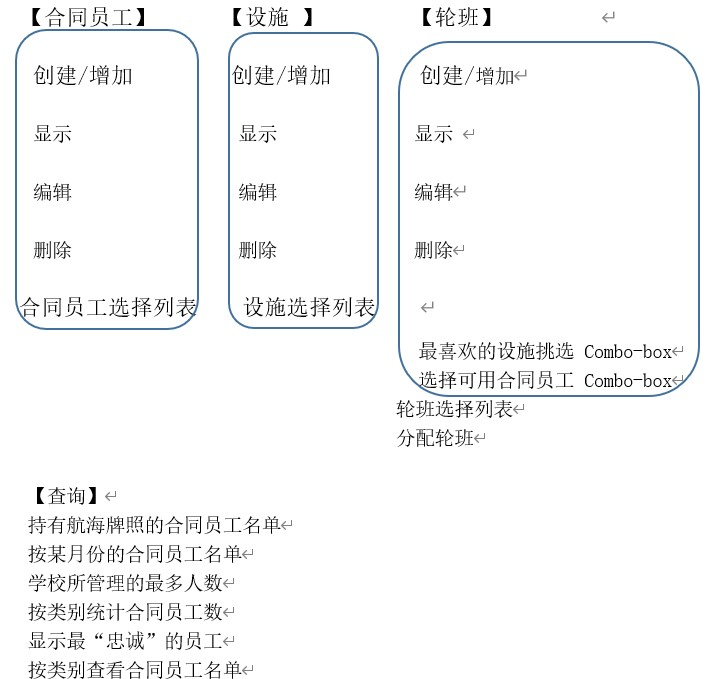
\includegraphics[width=10cm]{Ex1SoluScreenshot20220405115926.jpg}

%\href{文件:微信截图_20220412130822.jpg}{550px}

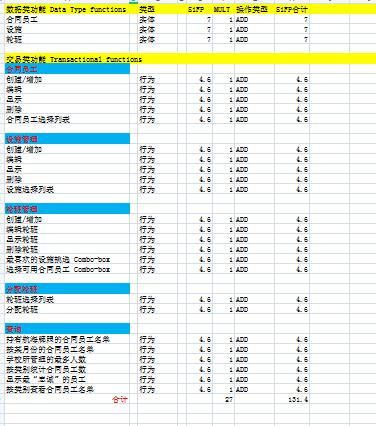
\includegraphics[width=10cm]{微信截图20220412130822.jpg}

%\href{文件:微信截图_20210330152654.png}{600px}

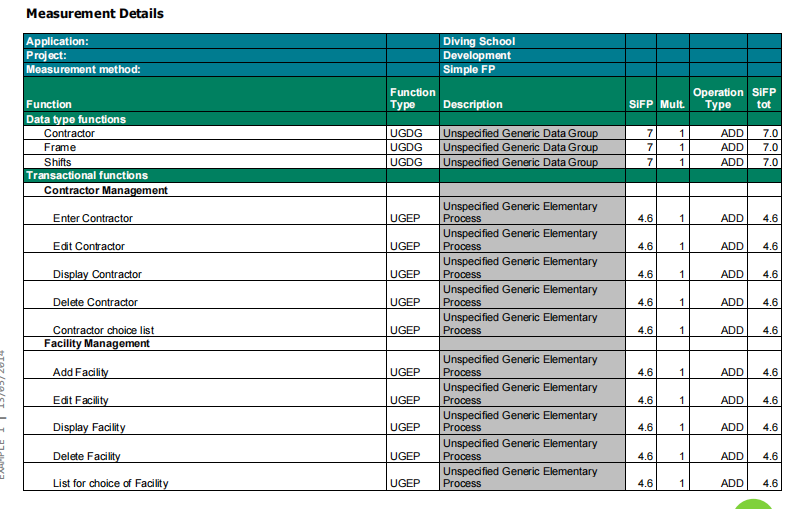
\includegraphics[width=10cm]{微信截图20210330152654.png}

%\href{文件:微信截图_20210330152702.png}{600px}

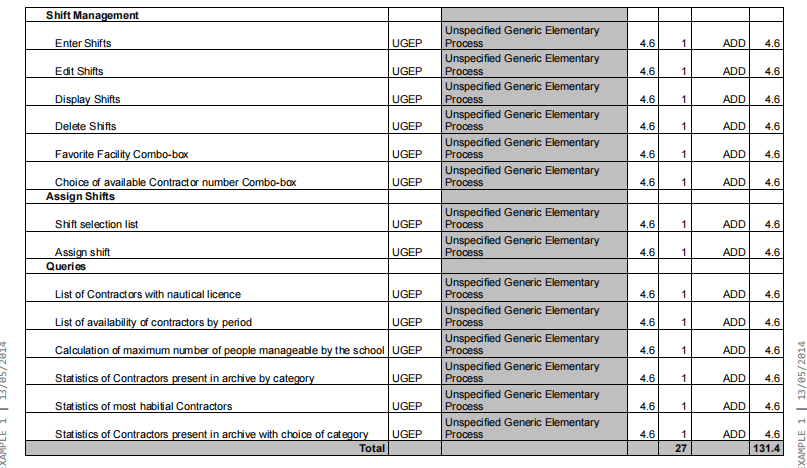
\includegraphics[width=10cm]{微信截图20210330152702.png}

\hypertarget{ux8ba1ux7b97ux529fux80fdux89c4ux6a21}{%
\subsubsection{计算功能规模}\label{ux8ba1ux7b97ux529fux80fdux89c4ux6a21}}

\begin{description}
\item[]
\begin{description}
\tightlist
\item[]
DSFP = ADD + CFP
\end{description}
\end{description}

因为没有数据转换,所以 CFP=0, 所以 DSFP = (110.4+21) +0 = 131.4 SiFP

因是首次开发, ASFP = ADD = 131.4 SiFP

\hypertarget{ux6f5cux6c34ux5b66ux6821femux9879ux76ee}{%
\subsection{2.潜水学校:FEM项目}\label{ux6f5cux6c34ux5b66ux6821femux9879ux76ee}}

\hypertarget{ux63cfux8ff0-1}{%
\subsubsection{描述}\label{ux63cfux8ff0-1}}

参照之前的潜水学校系统,对功能进行了增强,并提出了该软件的功能优化维护项目(FEM)。With
reference to the previously measured Diving School system, a Functional
Enhancement Maintenance Project (FEM) for the Software is proposed.

\hypertarget{ux529fux80fdux9700ux6c42-1}{%
\subsubsection{功能需求}\label{ux529fux80fdux9700ux6c42-1}}

\hypertarget{rf01-1}{%
\paragraph{RF01}\label{rf01-1}}

用户想要取消合同员工删除功能。The user wants to eliminate the Contractor
delete function.

\hypertarget{rf02-1}{%
\paragraph{RF02}\label{rf02-1}}

在短途潜水里, 在潜水设施管理中能管理船上医生的存在或缺失。The
presence/absence of a ship doctor during excursions must be managed in
the file DIVING FACILITIES.

\hypertarget{rf03-1}{%
\paragraph{RF03}\label{rf03-1}}

出于税收和安全原因,不再需要删除可用轮班这项功能 For tax and safety
reasons the function to delete availability shifts will no longer be
required.

\hypertarget{rf04-1}{%
\paragraph{RF04}\label{rf04-1}}

用户还需要管理课程参与者信息和他们参加的那个短途潜水信息:\\
*管理参与者的信息包括:参与者ID,姓,名,出生日期,潜水执照,执照日期。\\
参加短途潜水:参与者ID。轮班编号,出游日,天数,最终考试是/否通过\\
*用列表框 (包括:参与者ID,姓,名)来选择轮班中的参与者。\\
*使用原本应用程序中已经有的列表框选择轮班。\\
*用功能键将激活这功能,并最终生成错误信息/结果。

用功能键初始填充课程参与者信息,参与者信息源自以前参与者信息的备份数据。

The user also needs to manage the information of course Participants and
their enrollment in the excursion. The information managed will be for
Participants: Participant ID, LastName, FirstName, Date of Birth, diving
license, license date. To enroll in the excursion shift: Participant ID,
Shift ID, excursion date, duration, final examination passed
(YES/NO).Selection of the participants in an excursion shift will be
obtained by List Box on the Participant file, containing Participant ID,
FirstName, LastName. For Shift selection the List box already available
in the basic application will be used. A function key will activate the
function, and eventually generate an error/outcome message.

A functionality will be provided to populate initially the participant's
file with an already existent archive of past participants.

\hypertarget{rf05-1}{%
\paragraph{RF05}\label{rf05-1}}

用户还需要能够在课程结束时颁发出席证书给在短途潜水中登记的所有参与者。除了管理参与者基础数据外,还需要管理:参与者所登记的轮班、轮班日期、时长、教练的姓名和医生(如在场)的姓名。该功能使用原本应用程序中已经可用的功能:选择轮班。用功能键将激活这些功能,并最终生成错误/结果消息。The
user also needs to be able to issue at the end of the course a
certificate of attendance to all participants enrolled in an excursion.
The information to manage, in addition to the participant master data,
are: the excursion shift the participant is enrolled in, the date of the
excursion, the duration, the name of the instructor and of the doctor if
present. For Shift selection the List box already available in the basic
application will be used. A function key will activate the functions,
and eventually generate an error/outcome message.

\hypertarget{rf06}{%
\paragraph{RF06}\label{rf06}}

用户还需要能够向合同员工颁发``教员身份参与证书'',其中的信息除了基础数据外还包括:轮班ID、教练ID、出游日、船医(如果有的话)。对于轮班选择,将使用原本应用程序中已经有的列表框。用功能键将激活这功能,并最终生成错误信息/结果。

The user also needs to be able to issue a \textbf{Certificate of
participation as instructor} to Contractors, in which the information
will be, in addition to master data: Shift ID, Instructor ID, excursion
date, ship doctor if present. For Shift selection the List box already
available in the application will be used.A function key will activate
the functions, and eventually generate an error/outcome message.

\hypertarget{ux4f8bux5b50ux4e8c-ux7b54ux6848ux4e0eux89e3ux8bfb}{%
\subsection{例子二:
答案与解读}\label{ux4f8bux5b50ux4e8c-ux7b54ux6848ux4e0eux89e3ux8bfb}}

RF02 变动了潜水设施的内容,所以设施实体有变更。\\
因为设施的信息有变更,导致跟这实体相关的行为,包括新增、编辑、和展示这三行为都会有变更。

另外加了两个要管理的实体:

\begin{enumerate}
\tightlist
\item
  参与者
\item
  短途潜水
\end{enumerate}

不需要合同员工的删除功能,所以是个行为删除。

在参与者的管理,除了增加,改动,展示和删除四个功能以外,还有可以挑选参与者的下拉框功能。

两个证书的功能

\begin{enumerate}
\tightlist
\item
  给教练的证书
\item
  给参与者发证书
\end{enumerate}

对应每个短途潜水也需要有添加、改动、展示、删除的四功能。
那个删除轮班功能也被删掉了。

增加了两个实体 -\/-参与者 与 短途旅行登记\\
Q: 为什么短途旅行登记算一个实体?\\
A: 因它包括的信息都不能归入已有的 【参与者】 【合同员工】 【设施
】【轮班】实体里,例如那位参与者参加了那个班,考试分数等。
也可参考IFPUG关于ILF/EIF (实体)的识别要求;必须符合以下条件:

\begin{enumerate}
\tightlist
\item
  数据的集合必须是逻辑相关的并且是用户可以识别
\item
  这些数据或者控制信息必须是在本应用的边界内被维护
\end{enumerate}

总结:

\begin{itemize}
\tightlist
\item
  实体方面增加了2 实体; 设施实体有变更。
\item
  行为方面主要的在旅行方面增加了4 增删改查的功能和。5
  参与者的功能(因为在里面加了一个下拉框功能),增加了2
  证书功能。改动了设施的增加、编辑、和展示,三个行为,删掉了两个行为。
\end{itemize}

所以动态功能点是增加的功能点64.6 (=2x7 +(4+2+5)x4.6),变更 20.8
(=3x4.6),删除9.2 (=2x4.6),总共的动态简化功能点 94.6。

静态功能点依据上面练习一那的131.4,加上增加的功能点 64.6,减掉
删除功能点 9.2,得出变更后静态功能点 186.8。

%\href{文件:Ex2XlsScreenshot_2022-04-05_143941.jpg}{550px}

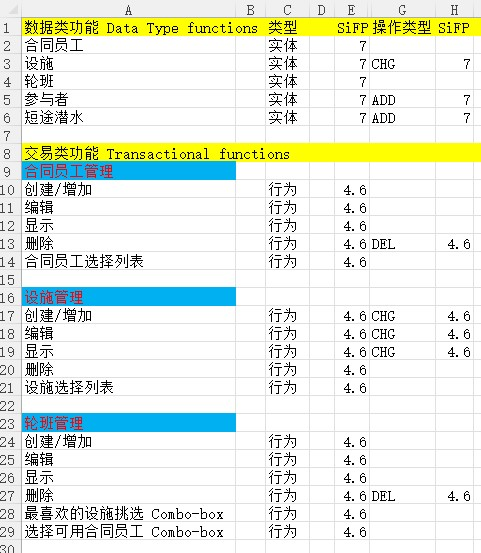
\includegraphics[width=10cm]{Ex2XlsScreenshot20220405143941.jpg}

%\href{文件:Ex2XlsPt2of2Screenshot_2022-04-05_143941.jpg}{550px}

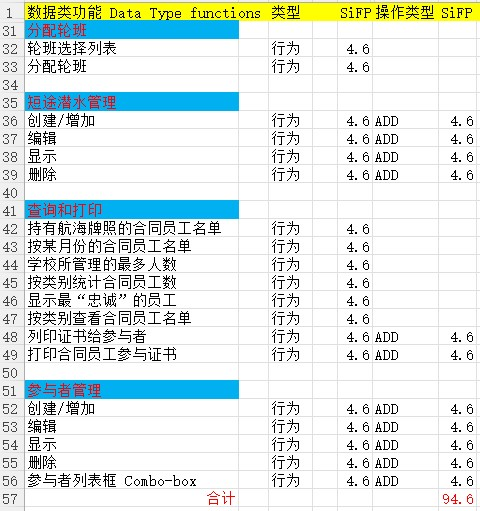
\includegraphics[width=10cm]{Ex2XlsPt2of2Screenshot20220405143941.jpg}

%\href{文件:微信截图_20210412093632.png}{600px}

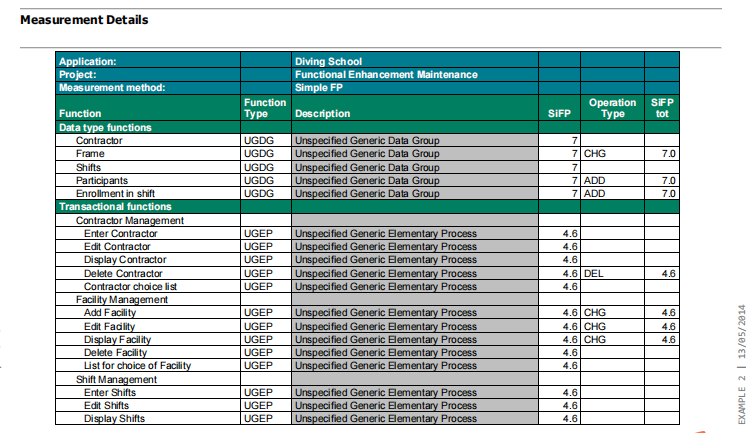
\includegraphics[width=10cm]{微信截图20210412093632.png}

%\href{文件:微信截图_20210412093858.png}{600px}

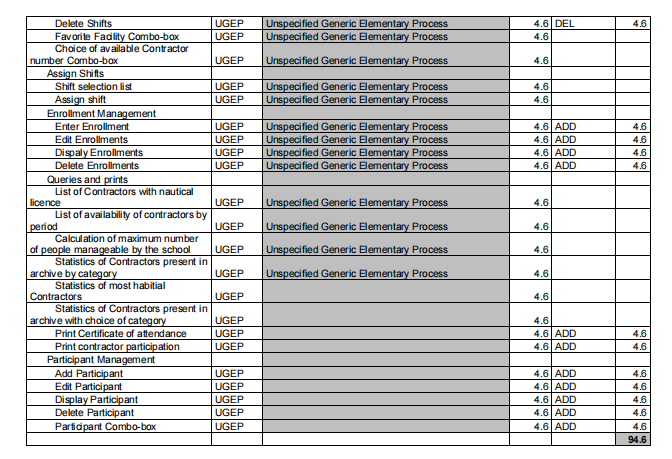
\includegraphics[width=10cm]{微信截图20210412093858.png}

\hypertarget{ux8ba1ux7b97ux529fux80fdux89c4ux6a21-1}{%
\subsubsection{计算功能规模}\label{ux8ba1ux7b97ux529fux80fdux89c4ux6a21-1}}

\begin{description}
\item[]
\begin{description}
\tightlist
\item[]
ESFP = ADD + CHG + DEL + CFP
\end{description}
\end{description}

因为有数据转换:初始填充课程参与者信息作为一个基本过程,所以 CFP=4.6

\begin{description}
\tightlist
\item[]
ESFP = (64.6 + 20.8 + 9.2) + 4.6 = 94.6 + 4.6 = 99.2 SiFP
\end{description}

软件开发后的静态功能点: ASFPA = ASFPB + ADD - DEL = 131.4 + 64.6 - 9.2
= 186.8 SiFP

\hypertarget{ux4e0eux56fdux9645ux529fux80fdux70b9ifpugux7684ux504fux5dee}{%
\subsection{与国际功能点(IFPUG)的偏差}\label{ux4e0eux56fdux9645ux529fux80fdux70b9ifpugux7684ux504fux5dee}}

例子:

\begin{itemize}
\tightlist
\item
  新开发某会计付款系统
\item
  实体: 包括管理 发票 ,付款,供货商。
\item
  行为:包括对每个实体的展示,增加,修改,和删除/取消
\item
  使用IFPUG 数 EI, EO, EQ, ILF, EIF
  每类的调整前功能点数,加起来得出调整前功能点数FP=82
  (如想多了解IFPUG如何计算复杂度,参考附件)
\item
  使用SiFP 估算实体和行为数,计算得出 FP=104
\end{itemize}

%\href{文件:FPA_S11.jpg}{500px}

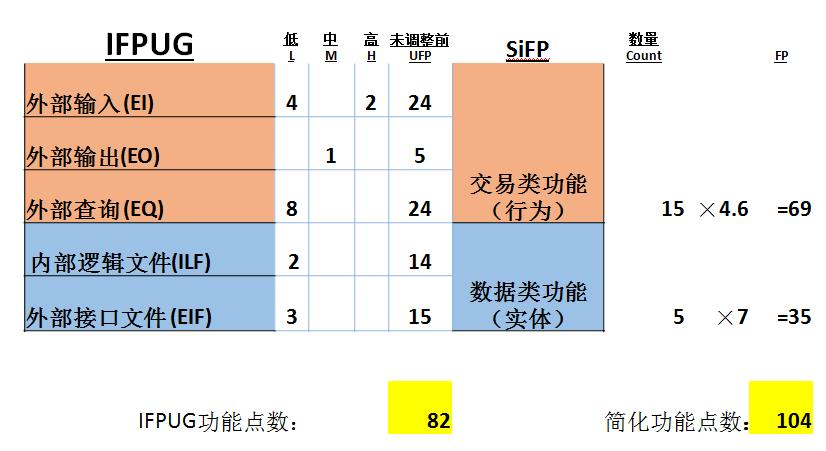
\includegraphics[width=10cm]{FPAS11.jpg}

\begin{itemize}
\tightlist
\item
  IFPUG / SiFP
  得出的实体数量,与行为数量都一样 (实体(=ILF+EIF)=5  行为
  (=EI+EO+EQ)=15)
\item
  因为简化功能点只是不区分实体与行为的复杂度(高中低),取平均值,原理一样,虽然个别估算有差异,但平均下来与IFPUG的估算没有结构性偏差
\end{itemize}

\hypertarget{ux7ec3ux4e60ux9898}{%
\section{练习题}\label{ux7ec3ux4e60ux9898}}

\hypertarget{ux65c5ux6e38ux670dux52a1-ux5f00ux53d1ux9879ux76eetourist-services---development-project}{%
\subsection{3.旅游服务-开发项目Tourist Services - Development
Project}\label{ux65c5ux6e38ux670dux52a1-ux5f00ux53d1ux9879ux76eetourist-services---development-project}}

\hypertarget{description}{%
\subsubsection{Description}\label{description}}

Wonder
Travel公司计划将其行程(Trips)管理系统自动化,该系统将连接各旅行预订系统
(travel Booking systems) 和行程路线(PV)系统。\\
The Wonder Travel company plans to automate its travel package (Trips)
management system, which will interface the travel Booking systems and
the Trip Routes (PV).

\hypertarget{functional-requirements}{%
\subsubsection{Functional requirements}\label{functional-requirements}}

该系统将由基于菜单界面的在线组件和定期运行的批处理组件组成。\\
The system will consist of an online component based on a menu interface
and a batch component that will run periodically.

\hypertarget{rf01-2}{%
\paragraph{RF01}\label{rf01-2}}

将使用行程包的行程码(ID)作为索引,存储数据。\\
行程(Trips)包括:

\begin{itemize}
\tightlist
\item
  行程码(ID)
\item
  行程路线编号(PV)
\item
  符合资格的导游姓名
\item
  行程类型(汽车、巴士、火车、飞机、游轮、混合)
\item
  计划版本数
\item
  版本频次(月、季等)\\
\end{itemize}

用户将从下拉列表中选择行程路线编号(PV code)
(来自行程路线(PV)文件),系统会 自动生成行程码 (Trip code)。 行程路线
Trip Routes (PV)
文件包含旅游区域(例如:北欧、北极、突尼斯、土耳其、希腊、美国、古巴和加勒比地区、日本、中国、埃及\ldots{}\ldots{}等等,信息都是由外部系统管理。\\
从导游注册文件中获得有资格的导游的名字,然后利用下拉列表来设置哪位导游有资格带哪个行程(Trip)。\\
版本状态字段将自动设置为``planned''(已策划)\\
行程类型将通过一个下拉列表来设置一些值,如``文化''或``休闲''或``宗教''等
使用功能键 (function
key)完成验证、一致性检查(编辑)和写入输入的数据,系统会按需要报错。\\
The travel package data will be stored in a Trips file using the Trip
code as the primary key.\\
The Trips will be entered using the following fields:

\begin{itemize}
\tightlist
\item
  Trip code (ID)
\item
  Trip Route code (PV)
\item
  names of tour guides qualified for the trip
\item
  trip type (by car, bus, train, airplane, cruise ship, mixed)
\item
  number of planned editions
\item
  frequency of editions (monthly, quarterly, etc.)\\
\end{itemize}

The Trip code will be set automatically while the PV code will be
selected from a drop-down list derived from the Trip Routes (PV) file
that contains the planned tourist areas (e.g.: Northern Europe, North
Pole, Tunisia, Turkey, Greece, United States, Cuba and the Caribbean,
Japan, China, Egypt, etc), managed externally.\\
The names of the Tour Guides qualified to make that kind of trip will be
set using a selection from a drop-down list obtained from the Guides
Register file.\\
The Edition status field will automatically be set to the value
"planned".\\
The trip type will be set using a selection from a drop-down list
showing some valid values such as "cultural" or "pleasure", or
"religious".\\
A function key will allow validation, congruence check (editing) and
writing the entered data. Error messages are generated if required.\\

\hypertarget{rf02-2}{%
\paragraph{RF02}\label{rf02-2}}

基于行程码(ID) (Trip code) 和功能键选择 Trips\\
Trips将显示与上一段中包含的相同数据,以及从PV文件中提取的数据,以及从RF07段中提到的导游注册文件中提取的导游的详细数据。\\
与前一节相同的Trips下拉列表将用于帮助用户进行选择。\\
如果trip文件中不存在搜索的行程码(ID),系统将报错。\\
The Trips will be displayed with the same data contained in the previous
paragraph and also with the data extracted from the PV file and the
detail data of the Guide extracted from the Guides Register file
mentioned in paragraph RF07. The selection will be based on the Trip
code and a function key.\\
A Trips drop-down list identical to that of the previous section will be
available to assist the user's selection. The system will generate an
error message if the trip code does not exist in the Trips file.

\hypertarget{rf03-2}{%
\paragraph{RF03}\label{rf03-2}}

RF01中包含的所有字段都可以修改 - 除了行程码(ID)(因为它是作为索引)。\\
版本状态字段只能通过 选择下拉列表中来更改, 只可以更改 包含``已提供
provided''和``已删除 deleted''值的内容。\\
无论如何,如更新版本状态字段将会自动更新:\\
* 余下可提供的版本数\#\#\\
::(\#\# 计划可提供版本数,减去已提供/删除的版本数)\\
也可用与RF01中相同的导游下拉列表挑选导游。\\
使用功能键 (function
key)完成验证、一致性检查(编辑)和写入输入的数据,系统会按需要报错。\\
All fields contained in paragraph RF01 can be modified except the Trip
code (since it is the key of the Trips file).\\
The edition status field can only be changed by making a selection from
a programmed drop-down list containing the values "provided" and
"deleted".\\
In any case, changing the Edition status field will be automatically
update the field:\\
* number of editions to provide\\
subtracting the number of editions provided and/or deleted from the
number of editions planned.\\
The same drop-down list of the Guides mentioned in paragraph RF01 will
be available.\\
A function key will validate and write the data. Error messages are
generated if required.\\

\hypertarget{rf04-2}{%
\paragraph{RF04}\label{rf04-2}}

选择行程码,按下功能键,即可取消行程。\\
使用RF01中提到相同下拉列表,来选择要删除的行程。如果Trip文件中不存在该行程码(ID),系统将报错。\\
也有取消确认消息。\\
A Trip can be cancelled by selecting the Trip code and pressing a
function key.\\
The same drop-down list of Trips referred to in paragraph RF01 will be
available to select a trip to be deleted. If the Trip code does not
exist in the Trips file, the system will generate an error message, and
a cancellation confirmation message.\\

\hypertarget{rf05-2}{%
\paragraph{RF05}\label{rf05-2}}

用户将能够查看属于某个行程路线(PV)的旅行版本的信息。用户必须输入行程码(ID)(Trip
code) 并按下功能键。选择的行程版本将显示以下数据:\\
*行程码(ID)

\begin{itemize}
\tightlist
\item
  行程描述
\item
  PV号
\item
  PV描述
\item
  导游姓名(所有符合资格的导游)
\item
  导游资格(所有有资格参加本次旅行的导游)
\item
  计划的版本数
\item
  版本的频率
\item
  提供的版本数
\item
  每个版:

  \begin{itemize}
  \tightlist
  \item
    版ID
  \item
    版日期
  \item
    版状态(已计划/提供/删除)
  \item
    已选择的导游\\
  \end{itemize}
\end{itemize}

行程描述和PV描述数据是从PV文件中提取。 用户也可以要求打印显示的信息。\\
The user will be able to view information about Trip editions that
belong to a certain Trip Route (PV). The user will have to enter the
Trip code and press a function key. The Trip editions selected will be
displayed with the following data:\\
*Trip code

\begin{itemize}
\tightlist
\item
  Trip description
\item
  PV code
\item
  PV description
\item
  Guide name (all guides qualified for this trip)
\item
  Guide qualification (all guides qualified for this trip)
\item
  number of editions planned
\item
  frequency of editions
\item
  number of editions to provide
\item
  for each edition

  \begin{itemize}
  \tightlist
  \item
    edition ID
  \item
    edition date
  \item
    edition status (planned/provided/deleted)
  \item
    selected guide\\
  \end{itemize}
\end{itemize}

The Trip description and PV description data is extracted from the PV
file. The user can also request printing the displayed data.

\hypertarget{rf06-1}{%
\paragraph{RF06}\label{rf06-1}}

由于WonderTravel提供的旅行具有季节性,通过选择行程代码(必须存在于旅行文件中)并输入版本日期(必须大于第一次输入的版本日期)来生成行程的版本。系统会自动生成唯一的版本码。版本的日期考虑了季节性相关的选择。\\
版本状态字段会自动设置为``planned''。一个功能键将激活数据的写入。如果需要,将生成错误消息。\\
Due to the seasonality of the trips offered by Wonder Travel, the
editions of a Trip are generated by selecting the Trip code (that must
be present in the Trips file) and entering the date of the edition (must
be a date greater than the edition date entered the first time). The
system will automatically generate a unique edition code. The dates of
the editions take into account seasonality related choices.\\
The edition status field will automatically be set to the value
"planned". A function key will activate the writing of the data. Error
messages are generated if required.

\hypertarget{rf07}{%
\paragraph{RF07}\label{rf07}}

有关导游的信息将以导游的姓名作为索引保存在导游登记簿中。\\
Information about Tour Guides will be kept in a Guides Register using
the Guide's name as the primary key.

\hypertarget{rf08}{%
\paragraph{RF08}\label{rf08}}

使用导游的姓名和功能键选择 ,
便可以显示导游信息。如果导游登记簿指南中不存在该导游,系统将生成一条消息。下拉列表与RF01的导游下拉列表相同。\\
The data of the Guide can be displayed. The selection will take place
using the name of the Guide and a function key. The system will generate
a message if the Guide does not exist in the Guides Register. The same
drop-down list of Guides as in paragraph RF01 will be available.

\hypertarget{rf09}{%
\paragraph{RF09}\label{rf09}}

除了导游的名称(因为它是索引),导游数据都可以更改。\\
可用于与RF01段相同的导游下拉列表,选择要修改数据的导游。\\
使用功能键 (function
key)完成验证、一致性检查(编辑)和写入输入的数据,系统会按需要报错。\\
Guide data can be changed, except for the name of the Guide (since it is
the key of the Guides Register file).\\
The same drop-down list of Guides as in paragraph RF01 will be available
to select the Guide to change.\\
A function key will allow editing and saving the data. Error messages
are generated if required.\\

\hypertarget{rf10}{%
\paragraph{RF10}\label{rf10}}

输入的旅行文件数据将通过一个文件发送到后台预订系统,更新 行程(Trips)
。信息来自行程(Trips) 文档及导游登记册(Guides Register) 。\\
The data entered in the Trips file will be sent via a file to the
Booking System to the Trip periodically. The information will be
obtained from the Trips file and from the Guides Register.

%\href{文件:Sifp_3_1.png}{文件:Sifp 3 1.png}

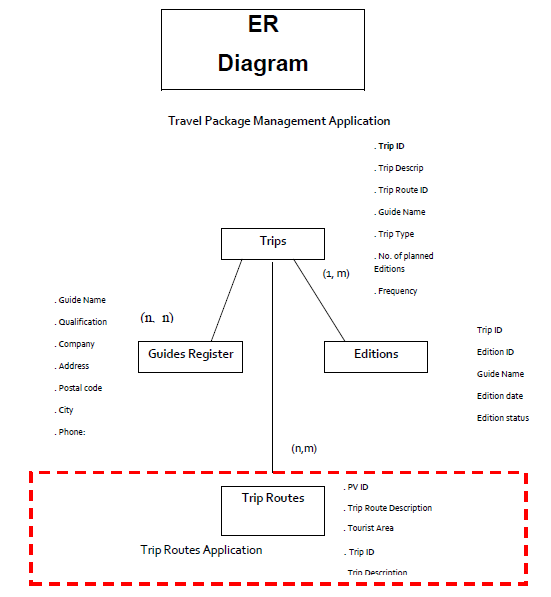
\includegraphics[width=10cm]{Sifp31.png}

%\href{文件:Sifp_3_2.png}{文件:Sifp 3 2.png}

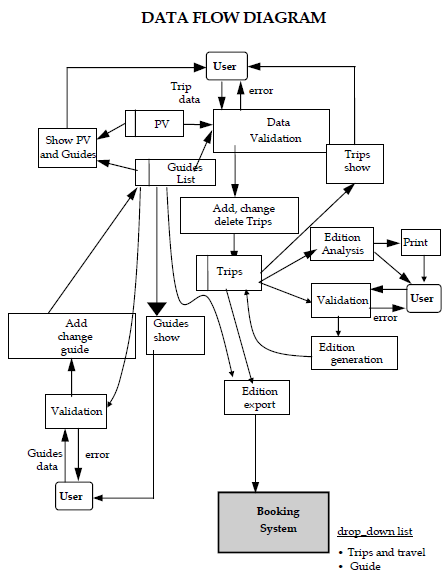
\includegraphics[width=10cm]{Sifp32.png}

\hypertarget{ux65c5ux6e38ux670dux52a1--femux9879ux76ee-tourist-services-fem-project}{%
\subsection{4.旅游服务- FEM项目 Tourist Services -- FEM
Project}\label{ux65c5ux6e38ux670dux52a1--femux9879ux76ee-tourist-services-fem-project}}

\hypertarget{description-1}{%
\subsubsection{Description}\label{description-1}}

基于以上例子3的旅游服务系统的基础上,提出以下软件功能增强与维护(FEM)\\
With reference to the previously measured Tourist Services system, a
Functional Enhancement Maintenance (FEM) Project for the Software is
proposed.

\hypertarget{functional-requirements-1}{%
\subsubsection{Functional
requirements}\label{functional-requirements-1}}

\hypertarget{rf01-3}{%
\subsubsection{RF01}\label{rf01-3}}

功能增强维护后,行程(Trips)管理系统必须显示在PV文件中旅行国家的当前政治局势的信息。\\
Information about the current political situation of the countries
included in the trip in the PV file must be displayed, following
functional enhancement maintenance of the Trip Routes system

\hypertarget{rf02-3}{%
\subsubsection{RF02}\label{rf02-3}}

有关导游经验的信息必须在导游登记档案的旅游领域(tourism)中处理。\\
Information about the experience of the tour guide must be handled in
the tourism field in the Guides Register file.

\hypertarget{rf03-3}{%
\subsubsection{RF03}\label{rf03-3}}

必须提供用户最多选择的行程/旅行套餐的统计数据。\\
Statistics about the travel packages most chosen by users must be
provided.

\hypertarget{rf04-3}{%
\subsubsection{RF04}\label{rf04-3}}

行程/旅游套餐必须送到相关政府部门备案。\\
Travel Packages must be sent to the Ministry of Foreign Affairs



